\documentclass{article}
\usepackage[utf8]

\usepackage[hidelinks]{hyperref} 

\usepackage{amsfonts}
\usepackage{amssymb}
\usepackage{xcolor}
\usepackage{tikz}
\usepackage{bbold}

\usepackage{stmaryrd}
\usepackage{float}

\usepackage{slashbox}

\usepackage{pdfpages}
\usepackage{svg}
\usepackage{subfig} %for placing tikzpicture in figs


%maths
\usepackage{mathtools}
\usepackage{amsmath}
\usepackage{amssymb}
\usepackage{amsfonts}

%Physics and chem
\usepackage{braket}
\usepackage{chemformula}

%tikzpicture
\usepackage{tikz}
\usepackage{scalerel}
\usepackage{pict2e}
\usepackage{tkz-euclide}
\usetikzlibrary{calc}
\usetikzlibrary{patterns,arrows.meta}
\usetikzlibrary{shadows}
\usetikzlibrary{external}

%pgfplots
\usepackage{pgfplots}
\pgfplotsset{compat=newest}
\usepgfplotslibrary{statistics}
\usepgfplotslibrary{fillbetween}

\usepackage{mathtools}% Loads amsmath


\title{Theoretische Physik 2}
\author{Momcilo Drljaca}
\date{\today}

\begin{document}

\maketitle
\raggedright

\section{Quantale Systeme mit endlichem Spektrum}

\color{cyan}

In diesem Kapitel wird geklärt was \textbf{Pauli Matrizen} sind und der Begriff \textbf{Spin} wird eingeführt. zunächst findet eine einführung über die Stern Gerlach Experimente stadt. Darus wird sich ergeben, dass ein \textbf{Superopsitionsprinzip} von nöten sein wird, und realtionen, denen gewisse Objekte (später $\sigma_i$) gehorchen müssen. Mit diesen Experimentellen Beobachtungen können die Pauli Matrizen konstruiert werden.

\color{black}
\subsection{Einführung}
\color{cyan}
Die EInführung gelingt am Besten mit Hilfe der \textbf{Stern Gerlach Experimente}. Diese sind auch Historisch gesehen für die entwicklung der Quantenmechanik von besonderer Relevanz.
\color{black}
\newline


Das \textbf{Stern Gerlach Experiment} besteht mindestens aus einer Teilchenquelle und einem \textbf{Stern Gerlach Apparat}\colro{blue} oder auch SG Apparat\color{black}. Abbildung \ref{Stern Gerlach Experiment} Zeigt den Aufbau. \color{cyan} Im Wesentlihen werden Teilchen in einem Ofen erhitzt und Kolimiert (gebündelt). Der Teilchenstrahl fliegt dann durch den Stern Gerlach Apparat und wird abgelenkt. Die abgelenkten Strahlen werden auf einem Schirm detektiert.\color{black}





\begin{figure}

\centering
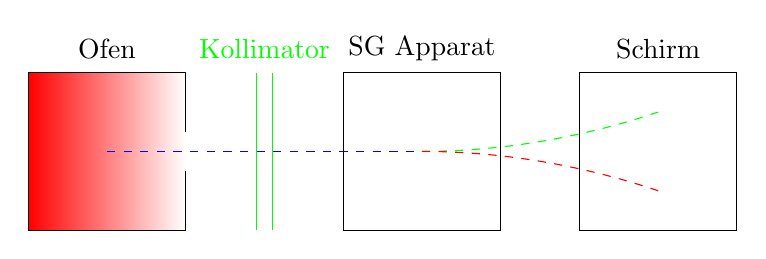
\begin{tikzpicture}
\shade[left color=red,right color=white] (0,0) rectangle (2,2) node at(1,2.3)  {Ofen};
\draw (0,0) --(2,0) -- (2,0.75);
\draw (2,1.25) -- (2,2) --(0,2) -- (0,0);
\draw[blue,dashed] (1,1) -- (5,1);
\draw[green,dashed] (5,1) parabola (8,1.5);
\draw[red,dashed] (5,1) parabola (8,0.5);
\draw[green] (2.9,0) -- (2.9, 2) node at(3,2.3) {Kollimator};
\draw[green] (3.1,0) -- (3.1, 2);
\draw (4,0) --(6,0) -- (6,2) -- (4,2) -- (4,0) node at(5,2.3) {SG Apparat};
\draw (7,0) --(9,0) -- (9,2) -- (7,2) -- (7,0) node at(8,2.3) {Schirm};
\end{tikzpicture}
\caption{Stern Gerlach Versuchsaufbau}
\label{Stern Gerlach Experiment}
\end{figure}




Der Stern Gerlach Apparat ist im Grunde nur ein inhomogenes Magnetfeld. \color{cyan} Ein Beispiel kann Abbildung \ref{Stern Gerlach Apparat (magn)} entnommen werden.\color{black}
\color{cyan}
Der Grund für die Notwendigkeit der Inhomogenität ist der, dass ein Magnetischer Dipol in einem homogenen Magnetfeld  (z.b Hufeisenmagnet)
sich nicht bewegt wenn er parallel zum Feld ausgerichtet ist.
\color{black}

\begin{figure}
\centering
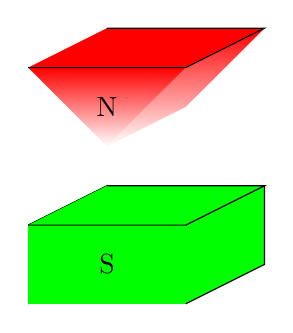
\begin{tikzpicture}
\shade[top color=red,bottom color=white] (1,2.5) -- (3,2.5) -- (2,1.5) -- (1,2.5);
\shade[top color=red,bottom color=white] (0,2) -- (2,2) -- (1,1) -- (0,2) node at(1,1.5)  {N};
\shade[top color=red,bottom color=white] (1,1) -- (2,2) -- (3,2.5) -- (2,1.5) -- (1,1);
\draw[fill=red,opacity=1] (0,2) -- (2,2) -- (3,2.5) -- (1,2.5);

\shade[top color=green,bottom color=green] (1,0.5) -- (3,0.5) -- (3,-0.5) -- (1,-0.5) -- (1,0.5);
\draw[fill=green,opacity=1] (0,0) -- (1,0.5) -- (1,-0.5) -- (0,-1);
\shade[top color=green,bottom color=green] (0,0) -- (2,0) -- (2,-1) -- (0,-1) -- (0,0) node at(1,-0.5)
 {S};
\draw[fill=green,opacity=1] (2,0) -- (3,0.5) -- (3,-0.5) -- (2,-1);
\draw[fill=green,opacity=1] (0,0) -- (2,0) -- (3,0.5) -- (1,0.5);
\end{tikzpicture}
\caption{Stern Gerlach Apparat.}
\label{Stern Gerlach Apparat (magn)}
\end{figure}
\newline


\color{cyan}
In der Regel werden beim Stern Gerlach Experiment \ce{Ag} Atome verwendet, da deren Elektronenkonfiguration für einen Gesamtspin des Atomes verantwortlich ist.
\newline

\color{black}
\subsubsection{Klassische Analyse}
\color{gray}
Wichtig ist im Folgenden der Fakt, dass durch die \textbf{Inhomogenität} des Magnetfeldes (insbesondere ist es nicht konstant in $z$-Richtung), die Ableitung $\partial_z \vec{B} \ne 0$ ist. Auserdem sollte klar sein, dass $\mu$ das \textbf{Magnetische Moment} (siehe \href{https://de.wikipedia.org/wiki/Magnetisches_Dipolmoment}{Magnetisches Moment Wikipedia}) ist, und $E_{pot} = \vec{\mu} \cdot \vec{B}$ gilt.
\color{black}

\begin{multiline}

 \color{white} \left\{ \color{black} H = \frac{p^2}{2m}-\vec{\mu}\cdot\vec{B}(\vec{r}) \right\}\color{black} \text{Hammiltonian} \\ \color{black}
 \text{Da alle anderen Ableitungen Null sind betrachte nur } z \text{ Richtung} \color{gray} \text{ dafür wird angenommen, die Atome fliegen genau durch die Mitte} \color{black}\\
\Rightarrow
F_z = - \nabla_z H = \vec{\nabla}_z\vec{\mu}\vec{B}(\vec{r})= \vec{\mu_z} \partial_z \vec{B}_z(z)
\end{multiline}
\newline

Wir erwarten naiv, dass $\vec{\mu}$ und damit auch $\vec{\mu}_z$ zufällig sind, und sich ein kontinuierlicher Verlauf auf dem Schirm Abzeichnet (etwa wie in Abbildung \ref{verlauf warscheinlichkeit naiv}).

\begin{figure}[h]
\centering
\begin{subfigure}
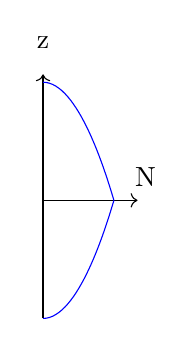
\begin{tikzpicture}
\draw[->] (0,0) -- (0,3.1) node at (0,3.5) {z};
\draw[->] (0,1.5) -- (1.2,1.5) node at (1.3,1.8) {N};
\draw[blue] (0,0) parabola (0.9,1.5);
\draw[blue] (0,3) parabola (0.9,1.5);
\end{tikzpicture}
\end{subfigure}
\begin{subfigure}
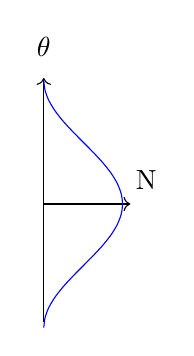
\begin{tikzpicture}
\draw[->] (0,0) -- (0,3.1) node at (0,3.5) {$\theta$};
\draw[->] (0,1.5) -- (1.1,1.5) node at (1.3,1.8) {N};
 \draw[scale=0.5,domain=-3.141:3.141,smooth,variable=\t, blue]
  plot ({cos(\t r) + 1},{\t + 3});
\end{tikzpicture}
\end{subfigure}

\caption{Erwarteter Verlauf ($N$ ist die Teilchenzahl an der Stelle vom Schim)}
\label{verlauf warscheinlichkeit naiv}
\end{figure}
\color{gray}
Man kann sich genauer überlegen was passiert, wenn der Winkel $\theta$, an Stelle von $z$ betrachtet wird.
\newline

dafür schreiben wir das Skalarprodukt äquivalent um 
\begin{equation}
 \vec{\mu} \cdot \vec{B} = |\vec{\mu}| \cdot |\vec{B}| \cdot \cos{(\theta)}
\end{equation}
Da es immernoch um einen Vektor geht, macht es Sinn davon auszugehen dass dieser (in der Einheitskugel) beliebig gedreht sein kann, also $\theta$ zufällig ist. $\theta$ ist also ein sinnvoller Parameter. Wenn $\theta$ gleichverteilt ist auf dem Intervall $[-\pi,\pi]$, und das Teilchen nährungsweise betragsmäsig proportional zur auf dieses wirkenden Karft verschoben wird, dann folgt die Warscheinlichkeitsverteilung auf dem Schirm der Gleichung \eqref{Warscheinlichkteitsverteilung nach theta}
\begin{equation}
p(\theta) = \frac{\cos{(\theta)}}{\int_{-\pi}^{\pi} \cos{(x)}dx} = \frac{\cos{(\theta)}}{2},
\label{Warscheinlichkteitsverteilung nach theta}
\end{equation}
Vergleiche Abbildung \ref{verlauf warscheinlichkeit naiv} (Verlauf nach Theta).
\newline

\color{black}
Nicht zu erwarten ist ein Diskreter Verlauf so wie in Abbildung \ref{Stern Gerlach Experiment} suggeriert wird. 
\newline

Definiere den \textbf{Operator} $\sigma_n$.
\newline

Dieser Operator liefert eine \textbf{Messgröße},\color{gray} wie jeder andere Operator auch\color{black}. Die Messgröße ist hierbei die Richtung $\vec{n}$, in die das Magnetische Moment $\vec{\mu}$ zeigt.\color{gray} also gilt $\vec{n}:=\frac{\vec{\mu}}{|\vec{\mu}|}$\color{black}. Dieser Operator misst also den \textbf{Spin} und wird in unserem Fall (Spin $\frac{1}{2}$ Teilchen) immer $\pm 1$ ergeben.
\newline

Die \textbf{Konvention} ordnet dann $\ket{n_+}$ dem Zustand \textit{Spin UP in Richtung $n$}, zu. Analog bedeutet $\ket{x_+}, \ket{z_+}$, \textit{Spin UP} in die entsprechende Richtung.
\newline

Die \textbf{Warscheinlichkeit} wird konventionell als $prob(...)$ oder $p(...)$ geschrieben.\color{cyan} Zum Beispiel
\begin{equation}
 prob(\sigma_z = \pm 1| \ket{z_+}) = 1.
 \label{warscheilichkeit reiner zust}
\end{equation}
\newline

Eine Reihe von Experimenten wird nun die Beobachtungen in der Realität demonstrieren, aus denen wir uns mit einigen wenigen \textbf{Postulaten}, eine Theorie aufbauen werden, um Vorhersagen über Quantale Systeme Treffen zu können.
\color{black}


\subsubsection{Experimente}

\textbf{Experiment 1} untersucht einen reinen Zustand, siehe Abbildung \ref{Exp1}.\color{gray}Die konvention ist hierbei so gewählt, dass \textbf{grüne Trajektorien} zu \textit{Spin \textbf{UP}} \textbf{Teilchen} gehören, und roten zu \textit{Spin DOWN}. Die \textbf{Dichte} des Strahles $\rho$ soll die Teilchendichte (oder Menge der Teilchen) darstellen (z.B ist ein gesplitteter Strahl mit $\rho = 0.5$ zu kennzeichnen.) \color{black}
\begin{figure}[H]
\centering
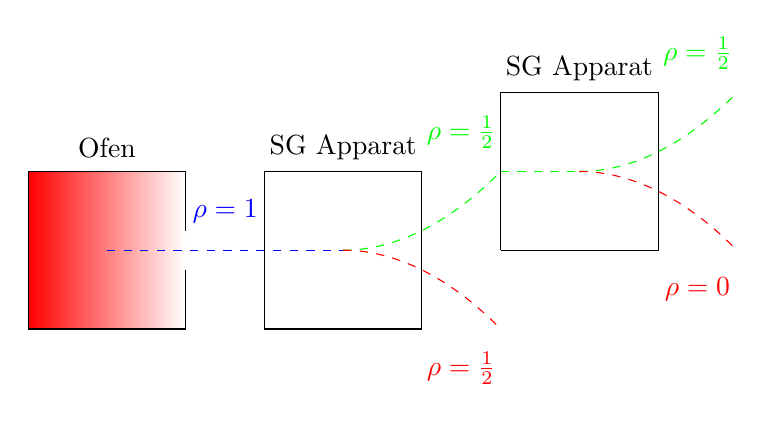
\begin{tikzpicture}

\shade[left color=red,right color=white] (0,0) rectangle (2,2) node at(1,2.3)  {Ofen}; % Ofen gradient
\draw (0,0) --(2,0) -- (2,0.75);												% Ofen unterer teil
\draw (2,1.25) -- (2,2) --(0,2) -- (0,0);										% Ofen oberer teil

\draw[blue,dashed] (1,1) -- (4,1) node at (2.5, 1.5) {$\rho = 1$};					% Teilchentrajektorie bis SG

\draw[green,dashed] (4,1) parabola (6,2) node at (5.5, 2.5) {$\rho =  \frac{1}{2}$};		% Teilchentrajektorie ab SG oben
\draw[green,dashed] (6,2) -- (7,2);									% Teilchentrajektorie ab SG oben
\draw[red,dashed] (4,1) parabola (6,0) node at (5.5, -0.5) {$\rho =  \frac{1}{2}$};		% Teilchentrajektorie ab SG unten

\draw (3,0) --(5,0) -- (5,2) -- (3,2) -- (3,0) node at(4,2.3) {SG Apparat};	% SG Apparat 1
\draw (6,1) --(8,1) -- (8,3) -- (6,3) -- (6,1) node at(7,3.3) {SG Apparat};	% SG Apparat 2

\draw[green,dashed] (7,2) parabola (9,3) node at (8.5, 3.5) {$\rho = \frac{1}{2}$};									% Teilchentrajektorie ab SG2 oben
\draw[red,dashed] (7,2) parabola (9,1) node at (8.5, 0.5) {$\rho = 0$};									% Teilchentrajektorie ab SG2 unten

\end{tikzpicture}
\caption{Experiment 1}
\label{Exp1}
\end{figure}

Damit folgt das Ergebniss aus \eqref{warscheilichkeit reiner zust}, also 
\begin{equation}
 p(\sigma_z = \pm 1| \ket{z_+}) = 1.
\end{equation}
\color{gray}
Es gilt sogar 
\begin{equation}
 p(\sigma_z = 1| \ket{z_+}) = 1.
\end{equation}
Hierbei setzt die obere Gleichung die Warscheinlichkeit vom Ereigniss $\sigma_z = 1$ oder $\sigma_z = -1$, unter der Bedingung dass der gemessene Zusatnad schon im Zusatnd $\ket{z_+}$ ist gleich mit der Zahl 1.
\color{black}




\newline


\textbf{Experiment 2} untersucht einen reinen Zustand,gemesen in verschiedene Richtungen. Siehe Abbildung \ref{Exp2}.

\begin{figure}[H]
\centering
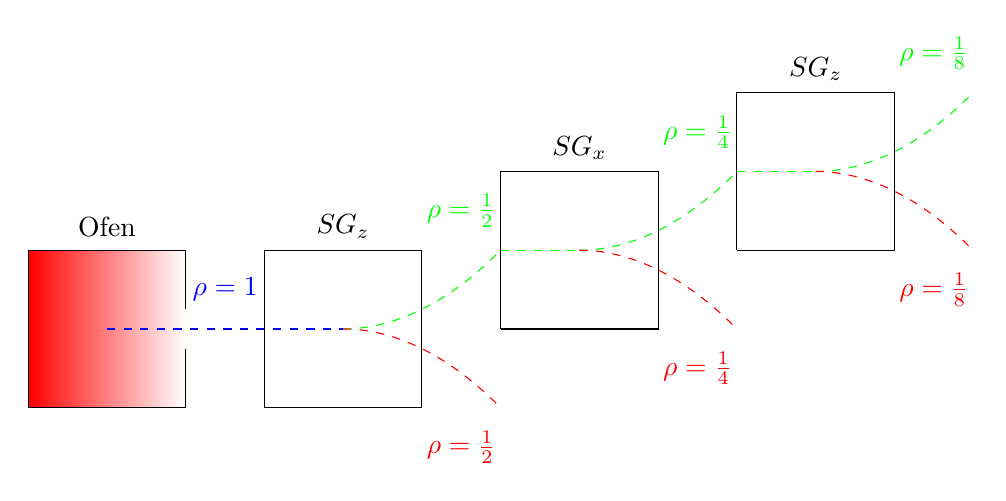
\begin{tikzpicture}

\shade[left color=red,right color=white] (0,0) rectangle (2,2) node at(1,2.3)  {Ofen}; % Ofen gradient
\draw (0,0) --(2,0) -- (2,0.75);												% Ofen unterer teil
\draw (2,1.25) -- (2,2) --(0,2) -- (0,0);										% Ofen oberer teil

\draw[blue,dashed] (1,1) -- (4,1) node at (2.5, 1.5) {$\rho = 1$};					% Teilchentrajektorie bis SG

\draw[green,dashed] (4,1) parabola (6,2) node at (5.5, 2.5) {$\rho =  \frac{1}{2}$};		% Teilchentrajektorie ab SG oben
\draw[green,dashed] (6,2) -- (7,2);									% Teilchentrajektorie ab SG oben
\draw[red,dashed] (4,1) parabola (6,0) node at (5.5, -0.5) {$\rho =  \frac{1}{2}$};		% Teilchentrajektorie ab SG unten

\draw (3,0) --(5,0) -- (5,2) -- (3,2) -- (3,0) node at(4,2.3) {$SG_z$};	% SG Apparat 1
\draw (6,1) --(8,1) -- (8,3) -- (6,3) -- (6,1) node at(7,3.3) {$SG_x$};	% SG Apparat 2
\draw (9,2) --(11,2) -- (11,4) -- (9,4) -- (9,2) node at(10,4.3) {$SG_z$};	% SG Apparat 3

\draw[green,dashed] (7,2) parabola (9,3) node at (8.5, 3.5) {$\rho = \frac{1}{4}$};	% Teilchentrajektorie ab SG2 oben
\draw[green,dashed] (9,3) -- (10,3);									% Teilchentrajektorie ab SG2 oben
\draw[red,dashed] (7,2) parabola (9,1) node at (8.5, 0.5) {$\rho = \frac{1}{4}$};		 % Teilchentrajektorie ab SG2 unten

\draw[green,dashed] (10,3) parabola (12,4) node at (11.5, 4.5) {$\rho = \frac{1}{8}$};	% Teilchentrajektorie ab SG3 oben
\draw[red,dashed] (10,3) parabola (12,2) node at (11.5, 1.5) {$\rho = \frac{1}{8}$};		 % Teilchentrajektorie ab SG3 unten

\end{tikzpicture}
\caption{Experiment 2}
\label{Exp2}
\end{figure}

\textit{Fazit}: Die Messung in $x$-Richtung hat den Zustand Verändert.


\newline


\textbf{Experiment 3} betrachtet Messung in beliebige Rcihtung. In Abbildung \ref{Exp3} ist die Messung in $z$-Richtung und dannach in $\vec{n}$-Richtung dargestellt.\color{gray} Dabei ist $\theta$ der kleinste Winkel zwischen den Vektoren $e_z$ und $\vec{n}$.\color{black}
\begin{figure}[H]
\centering
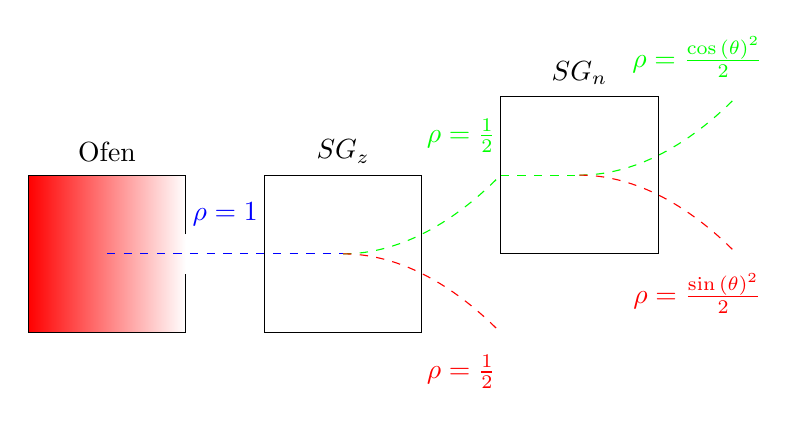
\begin{tikzpicture}

\shade[left color=red,right color=white] (0,0) rectangle (2,2) node at(1,2.3)  {Ofen}; % Ofen gradient
\draw (0,0) --(2,0) -- (2,0.75);												% Ofen unterer teil
\draw (2,1.25) -- (2,2) --(0,2) -- (0,0);										% Ofen oberer teil

\draw[blue,dashed] (1,1) -- (4,1) node at (2.5, 1.5) {$\rho = 1$};					% Teilchentrajektorie bis SG

\draw[green,dashed] (4,1) parabola (6,2) node at (5.5, 2.5) {$\rho =  \frac{1}{2}$};		% Teilchentrajektorie ab SG oben
\draw[green,dashed] (6,2) -- (7,2);									% Teilchentrajektorie ab SG oben
\draw[red,dashed] (4,1) parabola (6,0) node at (5.5, -0.5) {$\rho =  \frac{1}{2}$};		% Teilchentrajektorie ab SG unten

\draw (3,0) --(5,0) -- (5,2) -- (3,2) -- (3,0) node at(4,2.3) {$SG_z$};	% SG Apparat 1
\draw (6,1) --(8,1) -- (8,3) -- (6,3) -- (6,1) node at(7,3.3) {$SG_n$};	% SG Apparat 2

\draw[green,dashed] (7,2) parabola (9,3) node at (8.5, 3.5) {$\rho = \frac{\cos{(\theta)}^2}{2}$};									% Teilchentrajektorie ab SG2 oben
\draw[red,dashed] (7,2) parabola (9,1) node at (8.5, 0.5) {$\rho = \frac{\sin{(\theta)}^2}{2}$};									% Teilchentrajektorie ab SG2 unten

\end{tikzpicture}
\caption{Experiment 3}
\label{Exp3}
\end{figure}


\newline


\textbf{Experiment 4} untersucht Zusammenführung gemessener Strahlen. Siehe Abbildung \ref{Exp2}. Wichtiges Stichwort ist \textbf{Superposition}. \color{cyan} Vergleiche diesen Aufbau mit Experiment 2 in Abbildung \ref{Exp2}.\color{black}

\begin{figure}[H]
\centering
\begin{tikzpicture}

\shade[left color=red,right color=white] (0,0) rectangle (2,2) node at(1,2.3)  {Ofen}; % Ofen gradient
\draw (0,0) --(2,0) -- (2,0.75);												% Ofen unterer teil
\draw (2,1.25) -- (2,2) --(0,2) -- (0,0);										% Ofen oberer teil

\draw[blue,dashed] (1,1) -- (4,1) node at (2.5, 1.5) {$\rho = 1$};					% Teilchentrajektorie bis SG

\draw[green,dashed] (4,1) parabola (6,2) node at (5.5, 2.5) {$\rho =  \frac{1}{2}$};		% Teilchentrajektorie ab SG oben
\draw[green,dashed] (6,2) -- (7,2);									% Teilchentrajektorie ab SG oben
\draw[red,dashed] (4,1) parabola (6,0) node at (5.5, -0.5) {$\rho =  \frac{1}{2}$};		% Teilchentrajektorie ab SG unten

\draw (3,0) --(5,0) -- (5,2) -- (3,2) -- (3,0) node at(4,2.3) {$SG_z$};	% SG Apparat 1
\draw (6,1) --(8,1) -- (8,3) -- (6,3) -- (6,1) node at(7,3.3) {$SG_x$};	% SG Apparat 2
\draw (9,1) --(11,1) -- (11,3) -- (9,3) -- (9,1) node at(10,3.3) {$SG_z$};	% SG Apparat 3

\draw[green,dashed] (7,2) cos (8,3) node at (8.5, 3.5) {$\rho = \frac{1}{4}$};	% Teilchentrajektorie ab SG2 oben
\draw[green,dashed] (8,3) cos (9,2) node at (8.5, 3.5);	% Teilchentrajektorie ab SG2 oben
\draw[green,dashed] (9,2) -- (10,2);									% Teilchentrajektorie ab SG2 oben
\draw[red,dashed] (7,2) cos (8,1) node at (8.5, 0.5) {$\rho = \frac{1}{4}$};		 % Teilchentrajektorie ab SG2 unten
\draw[red,dashed] (8,1) cos (9,2);		 % Teilchentrajektorie ab SG2 unten

\draw[green,dashed] (10,2) parabola (12,3) node at (11.5, 3.5) {$\rho = \frac{1}{2}$};	% Teilchentrajektorie ab SG3 oben
\draw[red,dashed] (10,2) parabola (12,1) node at (11.5, 0.5) {$\rho = 0$};		 % Teilchentrajektorie ab SG3 unten

\end{tikzpicture}
\caption{Experiment 4}
\label{Exp4}
\end{figure}

\color{cyan}
Das Experiment in Abbildung \ref{Exp4} zeigt im gegensatz zum Experiment in Abbildung \ref{Exp2} nicht dass die \textbf{Messung der Zustände}, \textbf{nicht kommutativ} ist, sondern dass auch \textbf{Superposition} eine Rolle spielt.\color{gray} Der Grund für den Ausgang wird klarer, wenn die Zustände eines Atomes ausgeschrieben werden.
\begin{itemize}
  \item \textbf{Ofen - $SG_z$} sind die Zustände undefiniert.
  \item \textbf{$SG_z$-$SG_x$} betrachten wir nur Atome im Zustand $\ket{z_+}$.
  \item \textbf{$SG_X$-$SG_z$} Der Grund für den Ausgang ist, dass beim Messen in $x$ Richtung der obere Pfad von einem Vektor (der \textit{x-UP} entspricht, in $z$ Basis) $\frac{1}{2}(\ket{1}+\ket{0})$, untere von einem Vektor $\frac{1}{2}(-\ket{1}+\ket{0})$ durchlaufen wird. ($\ket{0}$ bedeutet $z$-UP). Die \textbf{Superposition} dieser beiden Vektoren ergibt den reinen $\ket{0}$ Zustand. dieser wird dann nach Messung in $z$-Richtung (vom letzten $SG$-Apparat) auch nicht mehr verändert.
  \textbf{Mann könnte annehmen:} hier werden die Zustände $\ket{z_+}$ \textbf{gemessen} mit dem \textbf{Spin Operator} $\hat{S}_x := \frac{\hbar}{2}\cdot \sigma_x$. Daraus ergibt sich (\textit{Vorgegriffen}) $\sigma_x \cdot \ket{z_+} = (\ket{0}\bra{1} + \ket{1}\bra{0}) \cdot \ket{0} = \ket{1}$ Diese Rechnung stimmt so aber nicht, weil der Operator $\hat{S}_x$ nur seine Eigenwerte Messen kann (wie jeder andere Operator auch), es kommt also als Ergebniss nur $\ket{+} oder \ket{-}$ raus, was in $z$-Basis $\ket{1}+\ket{0}$ und $-\ket{1}+\ket{0}$ ergibt (bis auf normierung). da beim messen in $x$-Richtung (ohne weitere informationen über den Spin in $x$), der Strahl am $SG$ genau halbiert wird, ist kürzen sich bei der Wiedervereinigung die $\ket{1}$-Anteile genau weg.
\end{itemize}
\color{black}

\newline


\textbf{Experiment 5} Versucht Überlegungen zu untersuchen, die Kontinuierliche Übergänge (zum beispiel wenn aus zwei Spalten einer wird) Betrachten. Siehe Abbildung \ref{Exp5a}, \ref{Exp5b} und \ref{Exp5c}. \color{cyan} Die Idee ist drei Versuchsteile Aufzubauen. dabei soll Teil b) in Teil c) kontinuierlich übergehen, indem einfach das $B$-Feld des $SG_x$-Apparates kontinuierlich schwächer gemacht wird.\color{black}

\textbf{Teil a)}
\begin{figure}[H]
\centering
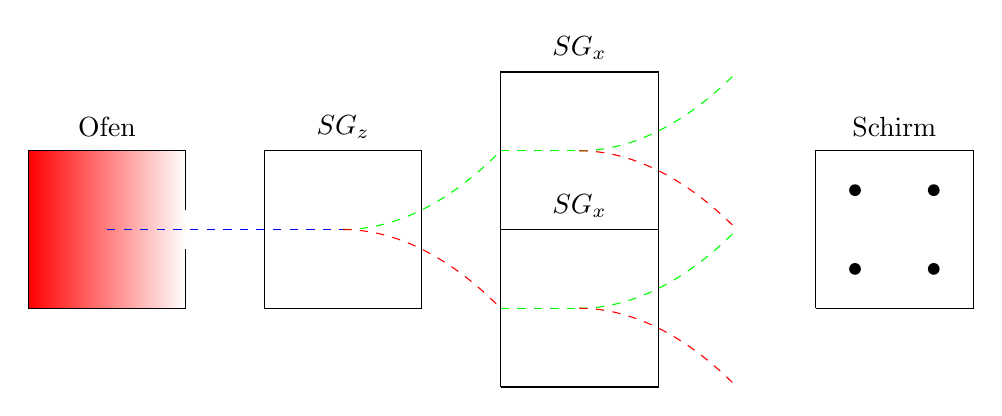
\begin{tikzpicture}

\shade[left color=red,right color=white] (0,0) rectangle (2,2) node at(1,2.3)  {Ofen}; % Ofen gradient
\draw (0,0) --(2,0) -- (2,0.75);												% Ofen unterer teil
\draw (2,1.25) -- (2,2) --(0,2) -- (0,0);										% Ofen oberer teil

\draw[blue,dashed] (1,1) -- (4,1) ;					% Teilchentrajektorie bis SG

\draw[green,dashed] (4,1) parabola (6,2) ;		% Teilchentrajektorie ab SG oben
\draw[green,dashed] (6,2) -- (7,2);									% Teilchentrajektorie ab SG oben
\draw[green,dashed] (6,0) -- (7,0);									% Teilchentrajektorie ab SG2 oben
\draw[red,dashed] (4,1) parabola (6,0) ;		% Teilchentrajektorie ab SG unten

\draw (3,0) --(5,0) -- (5,2) -- (3,2) -- (3,0) node at(4,2.3) {$SG_z$};	% SG Apparat 1
\draw (6,1) --(8,1) -- (8,3) -- (6,3) -- (6,1) node at(7,3.3) {$SG_x$};	% SG Apparat 2
\draw (6,-1) --(8,-1) -- (8,1) -- (6,1) -- (6,-1) node at(7,1.3) {$SG_x$};	% SG Apparat 3

\draw[green,dashed] (7,2) parabola (9,3) ;									% Teilchentrajektorie ab SG2 oben
\draw[red,dashed] (7,2) parabola (9,1) ;									% Teilchentrajektorie ab SG2 unten

\draw[green,dashed] (7,0) parabola (9,1) ;									% Teilchentrajektorie ab SG3 oben
\draw[red,dashed] (7,0) parabola (9,-1) ;									% Teilchentrajektorie ab SG3 unten
\draw (10,0) -- (12,0) -- (12, 2) -- (10,2) -- (10,0) node at(11,2.3) {Schirm};
\node at (10.5,0.5) [circle,fill,inner sep=1.5pt]{};
\node at (11.5,0.5) [circle,fill,inner sep=1.5pt]{};
\node at (10.5,1.5) [circle,fill,inner sep=1.5pt]{};
\node at (11.5,1.5) [circle,fill,inner sep=1.5pt]{};

\end{tikzpicture}
\caption{Experiment 5,a)}
\label{Exp5a}
\end{figure}
\color{black}

\textbf{Teil b)}.Analog zum Experiment in Abbildung \ref{Exp5a} wird noch ein Block an Stern gerlach Apparaten platziert um den Spin in $z$ Richtung zu messen. Vereinfacht dargestellt ist dieser Aufbau inm Experiment in Abbildung \ref{Exp5b} zu sehen.

\begin{figure}[H]
\centering
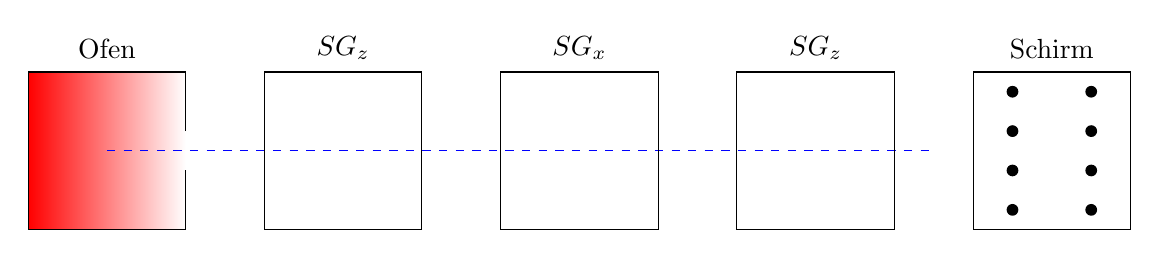
\begin{tikzpicture}

\shade[left color=red,right color=white] (0,0) rectangle (2,2) node at(1,2.3)  {Ofen}; % Ofen gradient
\draw (0,0) --(2,0) -- (2,0.75);												% Ofen unterer teil
\draw (2,1.25) -- (2,2) --(0,2) -- (0,0);										% Ofen oberer teil

\draw[blue,dashed] (1,1) -- (11.5,1) ;					% Teilchentrajektorie bis SG


\draw (3,0) --(5,0) -- (5,2) -- (3,2) -- (3,0) node at(4,2.3) {$SG_z$};	% SG Apparat 1
\draw (6,0) --(8,0) -- (8,2) -- (6,2) -- (6,0) node at(7,2.3) {$SG_x$};	% SG B 2
\draw (9,0) --(11,0) -- (11,2) -- (9,2) -- (9,0) node at(10,2.3) {$SG_z$};	% SG B 3



\draw (12,0) -- (14,0) -- (14, 2) -- (12,2) -- (12,0) node at(13,2.3) {Schirm};
\node at (12.5,0.25) [circle,fill,inner sep=1.5pt]{};
\node at (13.5,0.25) [circle,fill,inner sep=1.5pt]{};
\node at (12.5,1.25) [circle,fill,inner sep=1.5pt]{};
\node at (13.5,1.25) [circle,fill,inner sep=1.5pt]{};
\node at (12.5,0.75) [circle,fill,inner sep=1.5pt]{};
\node at (13.5,0.75) [circle,fill,inner sep=1.5pt]{};
\node at (12.5,1.75) [circle,fill,inner sep=1.5pt]{};
\node at (13.5,1.75) [circle,fill,inner sep=1.5pt]{};

\end{tikzpicture}
\caption{Experiment 5,b)}
\label{Exp5b}
\end{figure}


\textbf{Teil c)}.in Diesem Teil wird der Aufbau aus Abbildung \ref{Exp5b} übernommen, und lediglich das $B$-Feld eines $SG$ Apparates kontinuierlich verringert.\color{cyan} Die Frage ist nun, was gescheit mit den Punkten auf dem Schirm, bzw wie sieht ein kontinuierlicher Übergang vom Schirm-Bild aus Abbildung \ref{Exp5a} zu dem aus Abbildung \ref{Exp5c} (grau) aus ? \color{black}

\begin{figure}[H]
\centering
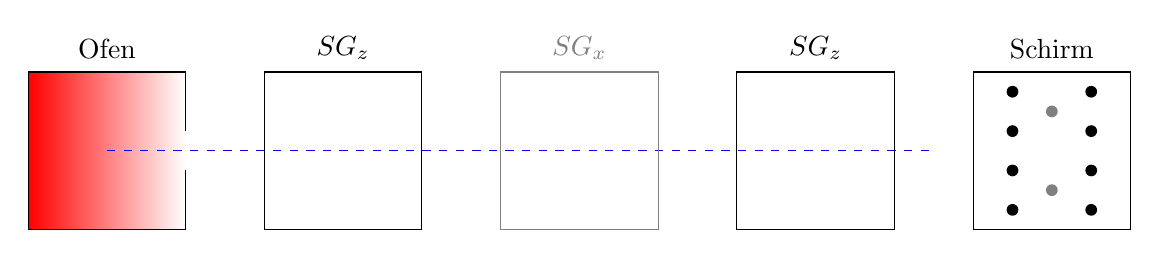
\begin{tikzpicture}

\shade[left color=red,right color=white] (0,0) rectangle (2,2) node at(1,2.3)  {Ofen}; % Ofen gradient
\draw (0,0) --(2,0) -- (2,0.75);												% Ofen unterer teil
\draw (2,1.25) -- (2,2) --(0,2) -- (0,0);										% Ofen oberer teil

\draw[blue,dashed] (1,1) -- (11.5,1) ;					% Teilchentrajektorie bis SG


\draw (3,0) --(5,0) -- (5,2) -- (3,2) -- (3,0) node at(4,2.3) {$SG_z$};	% SG Apparat 1
\draw[gray] (6,0) --(8,0) -- (8,2) -- (6,2) -- (6,0) node at(7,2.3) {$SG_x$};	% SG B 2
\draw (9,0) --(11,0) -- (11,2) -- (9,2) -- (9,0) node at(10,2.3) {$SG_z$};	% SG B 3



\draw (12,0) -- (14,0) -- (14, 2) -- (12,2) -- (12,0) node at(13,2.3) {Schirm};
\node at (12.5,0.25) [circle,fill,inner sep=1.5pt]{};
\node at (13.5,0.25) [circle,fill,inner sep=1.5pt]{};
\node at (12.5,1.25) [circle,fill,inner sep=1.5pt]{};
\node at (13.5,1.25) [circle,fill,inner sep=1.5pt]{};
\node at (12.5,0.75) [circle,fill,inner sep=1.5pt]{};
\node at (13.5,0.75) [circle,fill,inner sep=1.5pt]{};
\node at (12.5,1.75) [circle,fill,inner sep=1.5pt]{};
\node at (13.5,1.75) [circle,fill,inner sep=1.5pt]{};
\node at (13,0.5) [circle,fill,inner sep=1.5pt, gray]{};
\node at (13,1.5) [circle,fill,inner sep=1.5pt, gray]{};


\end{tikzpicture}
\caption{Experiment 5,b)}
\label{Exp5c}
\end{figure}

\newline

\color{gray}
Die Punkte sollten in $x$-Richtung zueinander rücken, bis nur noch die $z$-Richtung die Punkte von einander unterscheidet. Dann springen sie auf das (in Abbildung \ref{Exp5c}) graue Bild.\color{black}

\subsubsection{Pauli Matrizen und Konstruktion vom Spin Operator}
\color{cyan}
Im folgenden Abschnitt wird Versucht einen \textbf{Spin Operator} zu konstruieren, mit dem Wissen, dass die Experimente des Vorherigen Abschnittes gelifert haben (Operator Theorie ist teilweise für das Verständniss Vorrausetzung). 
\newline

\color{black}
Wir konnten im Experiment aus Abbildung \ref{Exp1} beobachten, dass die Folgende Gleichung für einen Spin Operator in $z$-Richtung $\hat{S}_z$ und ein Teilchen im $\ket{\sigma}$ Zustand (der entweder $\ket{z_+}$ oder $\ket{z_-}$ entspricht), gelten muss

\begin{equation}
\hat{S}_z \ket{\sigma} = \sigma \cdot\frac{\hbar}{2}\cdot  \ket{\sigma} 
\end{equation}

 wobei $\sigma$ einfach eine Konstante aus $\mathbb{C}$ ist (und somit ein \textbf{Eigenwert} des Operators $\hat{S}_z$).
\newline
 
  Der Wert von $\sigma$ ist laut den Experimenten $\sigma = +1$ falls $\ket{\sigma} = \ket{z_+}$ und  $\sigma = -1$ falls $\ket{\sigma} = \ket{z_-}$.
  \newline
  
  
 Auserdem ist ein Teilchen scheinbar \textbf{immer} in einem Zustand (nicht $\sigma = 0$), dass sieht man auch in Abbildung \ref{Exp1}, da die Mitte vom Schirm leer bleibt.
 Daraus folgt dass $\bra{z_i}\ket{z_k} = \delta_{i,k}$ (also besteht praktisch der zustand $\ket{z_+}$ zu 0 prozent aus $\ket{z_-}$, da sonnst deren Skalarprodukt nicht Null währe). Damit gilt
\begin{equation}
 \bra{\sigma'}\hat{S}_z\ket{\sigma} = \sigma \frac{\hbar}{2} \braket{\sigma'|\sigma} = \sigma \frac{\hbar}{2} \delta_{\sigma,\sigma'}
\end{equation}
Daraus ergibt sich die \textbf{eindeutige} Matrixdarstellung der Spinoperators $\hat{S}_z$ in $z$-Basis zu 
\newline


\begin{align}\hat{S}_z = \begin{tabular}{ | c | c | c | }
       \hline     
       \backslashbox{\sigma'}{\sigma} & +1 & -1 \\ \hline 
       +1 & $\frac{\hbar}{2}$ & 0 \\ \hline     
       -1 & 0 & $-\frac{\hbar}{2}$ \\     
       \hline  
  \end{tabular}= \frac{\hbar}{2} \cdot \begin{pmatrix}
1& 0 \\
0& -1 \\
\end{pmatrix}\end{align}

Analog schauen wir uns nun den Operator $\hat{S}_x$ an. Dieser wirkt analog zum $\hat{S}_z$ Operator, auf die Zustände $\ket{x_+}$ und $\ket{x_-}$ und bildet ab auf 
\begin{align}
\hat{S}_x \ket{x_+} = \ket{x_+},\\
\hat{S}_x \ket{x_-} = -\ket{x_-}
\end{align}
Damit folgt mit der \textbf{Spektraldarstellung}
\begin{align}
\hat{S}_x = (\ket{x_+}\bra{x_+}- \ket{x_-}\bra{x_-})\\
\Rightarrow \bra{\sigma'}\hat{S}_x\ket{\sigma} = \bra{\sigma'}(\ket{x_+}\bra{x_+}- \ket{x_-}\bra{x_-})\ket{\sigma}
\end{align}
nun Überlegen wir was gescheit falls $\sigma = \sigma'$, dann ergibt sich $\bra{\sigma'}\hat{S}_x\ket{\sigma}=\bra{\sigma}\ket{x_+}\bra{x_+}\ket{\sigma}- \bra{\sigma}\ket{x_-}\bra{x_-}\ket{\sigma}) = 0$.\color{gray} Für diese Gleichheit benötigt man den Fakt, dass $\ket{\sigma'} = \ket{\sigma} = \ket{z_+}$ dem Fall entspricht, bei dem ein Zustand $\ket{z_+}$ in $x$-Richtung geemessen wird, und dannach in $\ket{z_+}$ Richtung projeziert (da genau die Hälfte des Strahles nach $x$-Messung, im $\ket{z_+}$ Zustand ist, ist der Nummerische Wert dieser Projektion $0.5$ [analog mit $\ket{z_-}$; 0.5]) Es folgt $0.5 - 0.5 = 0$.\color{black} Also sieht $\hat{S}_x$ schon mal so aus $\begin{pmatrix}
0& a \\
b& 0 \\
\end{pmatrix}$.
\newline
Analog muss überlegt werden, dass im Falle (a) $\ket{\sigma} = \ket{z_-}, \ket{\sigma'} = \ket{z_+}$, $\bra{\sigma'}\hat{S}_x\ket{\sigma} = \braket{z_+|x_+}\braket{x_+|z_-}- \braket{z_+|x_-}\braket{x_-|z_-}$ einem Fall aus dem Experiment in Abbildung \ref{Exp1} entspricht, und zu $0.5-(-0.5)$ evaluiert. analog für (b).
Es folgt
\begin{equation}
\hat{S}_x = \frac{\hbar}{2}\begin{pmatrix}
0& 1 \\
1& 0 \\
\end{pmatrix}.
\end{equation}

Für $\hat{S}_y$ (und eine saubere herleitunge von (a) und (b) für $\hat{S}_x$), muss mit Gruppentheoreitschen Argumenten gearbeitet werden (nicht weiter verfogt).
\newline

Es ergibt sich 
\begin{equation}
\hat{S}_y = \frac{\hbar}{2}\begin{pmatrix}
0& -i \\
i& 0 \\
\end{pmatrix}
\end{equation}

Die Pauli Matrizen erfüllen (nach konstruktion) die Kommutatorrelation
\begin{equation}
	[\sigma_i,\sigma_j]= 2i\epsilon_{i,j,k}\sigma_k
\end{equation}

Wichtig ist noch nazumerken, dass die Paulimatrizen in $z$-Basis nicht als vollständige Darstellung des $\hat{S}$ Operators gesehen werden können. Die Darstellung von $\hat{S}_x$ in $z$-Basis (also $\frac{\hbar}{2}\sigma_1$) ist nütlich, da ihre Eigenvektoren $\frac{1}{\sqrt{2}}\begin{pmatrix}
1 \\
1 \\
\end{pmatrix}$ und $\frac{\hbar}{\sqrt{2}}\begin{pmatrix}
1 \\
-1 \\
\end{pmatrix}$ die Messergebnisse repräsentieren, und angeben wie der Anteil der $\ket{z_+}$ und $\ket{z_-}$ Zustände darin ist. \color{cyan} Zum beispiel ist im $\ket{x_+}$ Zustand (in $z$-Basis ist das der Eigenvektor $\frac{1}{\sqrt{2}}\begin{pmatrix}
1 \\
1 \\
\end{pmatrix}$) gleichviel von $\ket{z_+}$ und $\ket{z_-}$ enthalten (undswar \braket{z_+|x_+} =
$\begin{pmatrix}
1 \\
0 \\
\end{pmatrix}
 \cdot \frac{1}{\sqrt{2}}\begin{pmatrix}
1 \\
1 \\
\end{pmatrix} = \frac{1}{\sqrt{2}}$
und 
\braket{z_-|x_+} =
$\begin{pmatrix}
0 \\
1 \\
\end{pmatrix}
 \cdot \frac{1}{\sqrt{2}}\begin{pmatrix}
1 \\
1 \\
\end{pmatrix} = \frac{1}{\sqrt{2}}$
).\color{black}

\ection{Mathematische Struktur}
\color{cyan}In diesem Abschnitt soll die Vektorraumstruktur des Hilbertraumes verdeutlicht werden\color{black}

\subsection{Definition Hilbertraum}
Ein Hilbertraum ist ein reeller oder komplexer Vektorraum $\mathcal{H}$ mit einem Skalarprodukt $\braket{.|.}$, der vollständig bezüglich der durch das Skalarprodukt induzierten Norm ist, in dem also jede Cauchy-Folge konvergiert.

\newline

Es gilt 
\begin{equation}
\braket{u|\lambda v} = \lambda \braket{u|v} \text{ und } \braket{\lambda u|v} = \bar{\lambda}\braket{u|v}
\end{equation}

\color{cyan}
Insbesondere kann der Vektorraum unbeschänkte Dimension haben, zum Beispiel sind manche Funktionenräume solche Hilberträume.
\color{black}

\subsection{Konvention Dirac Noatation}
Dirac Noatation setzt Bra-Ket-Schreibweiße vorraus und notiert damit einen \textbf{Vektor} z.B als $\ket{x}$ (anstadt eine Basis zu wählen und diesen Vektor als splatenvektor zu schreiben).
\textbf{Operatoren} werden als Buchstaben Notiert . Eine Messung (Vektoren [Zustände] werden auf den Operator geschickt) kann dann so aussehen
\begin{equation}
\braket{x|A|\phi} =  \braket{A^\dag|x\phi} = \braket{xA|\phi}
\end{equation}
\color{cyan} Insbesondere hat die platzierung des symbols " $ \vline$ " keine besondere Bedeutung, der linke und rechte Teil der oberen Gleichung sind exakt gleichbedeutend.
\color{black}
Eine Übersicht der korrespondierenden Bra's zu bestimmten kets findet sich in Tabelle \ref{tab:bra ket not}

\begin{center}
\begin{tabular}{  c | c  }    
       Bra & Ket  \\ \hline 
       $\ket{\phi}$ & $\bra{\phi}$ \\ \hline     
       $\ket{c\cdot \phi}$ & $c^*\bra{\phi}$ \\  \hline
       $\ket{A\phi}$ & $\bra{A^\dag} = \bra{\phi}A^\dag$    
       \hline  
       \caption{Bra Ket Veranschaulichung}
       \label{tab:bra ket not}
  \end{tabular}
 \end{center}


\subsection{Rabi Oszillation}
Ein oszillieredes Magnetfeld kann dargestellt werden als
\begin{equation}
	\vec{B} = B_z \vec{e}_z + B_1[\cos{(\omega_1 t)} \vec{e}_x + \sin{(\omega_1 t)} \vec{e}_y}] = 
	\begin{pmatrix}
           B_z \\
           B_1 \cdot \cos{(\omega_1 t)} \\
           B_1 \cdot \sin{(\omega_1 t)}
         \end{pmatrix}
\end{equation}
Die Energie des Magnetfeldes auf einen Spin, der in Richtung des Feldes zeigt berechnet sich aus der klassischen formel 
\begin{equation}
 E =  -\vec{\mu} \cdot \vec{B}
\end{equation}
auf das \textbf{Magnetische Moment} $\mu$ kommen wir mit den \textbf{Pauli Matrizen}. 
\color{cyan}Ist zum Beispiel ein Teilchen im Zustand $\ket{z_+}$, so ist dessen Spin gleich \color{black}$\frac{\hbar}{2} = \hat{S}_z \ket{z_+} = \frac{\hbar}{2}\sigma_z \ket{z_+}$\color{cyan}. 
Im \textbf{klassischen Fall} würden wir $\vec{\mu} = \frac{q}{2m}\cdot \vec{L}$ benutzen 
(bzw bei von Massenverteilulng verscheidener Ladungsverteilung:  $\vec{\mu} = g_m \cdot\frac{q}{2m}\cdot \vec{L}$). 
Mann kann aber experimentell belegen, dass selbst Punktteilchen einen Spin besitzen.
\color{black}
Damit ergibt sich unser Hammiltonian als \textbf{Energie-Operator} zu
\begin{equation}
	H = \sum_{i \in \{x,y,z\}}-\mu_i \cdot B_i	\\
	\Rightarrow H = \frac{\hbar \omega_0}{2}\sigma_z + \frac{\hbar \omega_1}{2}[\cos{(\omega_1 t)}\sigma_x + \sin{(\omega_1 t)}\sigma_y]
\end{equation}

\color{red}Notiz: an dieser Stelle ergab sich au der Vorlesung nicht direkt, weshalb das \textbf{Minus} Vorzeichen beim Hammiltonian im Folgenden fehlt.\color{black}

Wegen der \textbf{Schrödinger Gleichung} folgt
\begin{align*}
i\hbar \partial_t \ket{\Psi} &= H \ket{\Psi} \\
\Rightarrow i \hbar \partial_t \begin{pmatrix}
c_+(t) \\
c_-(t) \\
\end{pmatrix}
&= 
\hbar\cdot \frac{\omega}{2} \begin{pmatrix}
0 & cos{(\omega t)} - i\sin{(\omega t)} \\
cos{(\omega t)} + i\sin{(\omega t)} & 0 \\
\end{pmatrix}\cdot\begin{pmatrix}
c_+(t) \\
c_-(t) \\
\end{pmatrix}
\end{align*}
Diese Glechung wird gelößt vom Vektor 
\begin{equation}
	\begin{pmatrix}
	e^{}\\
	\cos{(\omega t)} + \sin{(\omega) t}
	\end{pmatrix}
\end{equation}






\end{document}